
\documentclass{article}
\usepackage{graphicx}
\graphicspath{ {./images/} }
\usepackage[landscape]{geometry}
\usepackage{url}
\usepackage{multicol}
\usepackage{amsmath}
\usepackage{esint}
\usepackage{amsfonts}
\usepackage{tikz}
\usetikzlibrary{decorations.pathmorphing}
\usepackage{amsmath,amssymb}

\usepackage{colortbl}
\usepackage{xcolor}
\usepackage{mathtools}
\usepackage{amsmath,amssymb}
\usepackage{enumitem}
\makeatletter

\newcommand*\bigcdot{\mathpalette\bigcdot@{.5}}
\newcommand*\bigcdot@[2]{\mathbin{\vcenter{\hbox{\scalebox{#2}{$\m@th#1\bullet$}}}}}
\makeatother

\title{Algorithms II Cheat Sheet}
\usepackage[brazilian]{babel}
\usepackage[utf8]{inputenc}

\advance\topmargin-.8in
\advance\textheight3in
\advance\textwidth3in
\advance\oddsidemargin-1.5in
\advance\evensidemargin-1.5in
\parindent0pt
\parskip2pt
\newcommand{\hr}{\centerline{\rule{3.5in}{1pt}}}
%\colorbox[HTML]{e4e4e4}{\makebox[\textwidth-2\fboxsep][l]{texto}
\begin{document}

\begin{center}{\huge{\textbf{Algorithms II Cheat Sheet}}}\\
\end{center}
\begin{multicols*}{3}

\tikzstyle{mybox} = [draw=black, fill=white, very thick,
    rectangle, rounded corners, inner sep=10pt, inner ysep=10pt]
\tikzstyle{fancytitle} =[fill=black, text=white, font=\bfseries]

%------------ tips ---------------
\begin{tikzpicture}
\node [mybox] (box){%
    \begin{minipage}{0.3\textwidth}
    Apply an algorithm you know in a clever way, don't write a new algorithm.

    \end{minipage}
};
%------------ tips Header ---------------------
\node[fancytitle, right=10pt] at (box.north west) {Tips};
\end{tikzpicture}


%------------ Set notation ---------------
\begin{tikzpicture}
\node [mybox] (box){%
    \begin{minipage}{0.3\textwidth}
    $A \in [10] \equiv A \in [1..10]$
    \end{minipage}
};
%------------ Set notation Header ---------------------
\node[fancytitle, right=10pt] at (box.north west) {Set notation};
\end{tikzpicture}
    
%------------ Big O ---------------
\begin{tikzpicture}
\node [mybox] (box){%
    \begin{minipage}{0.3\textwidth}
        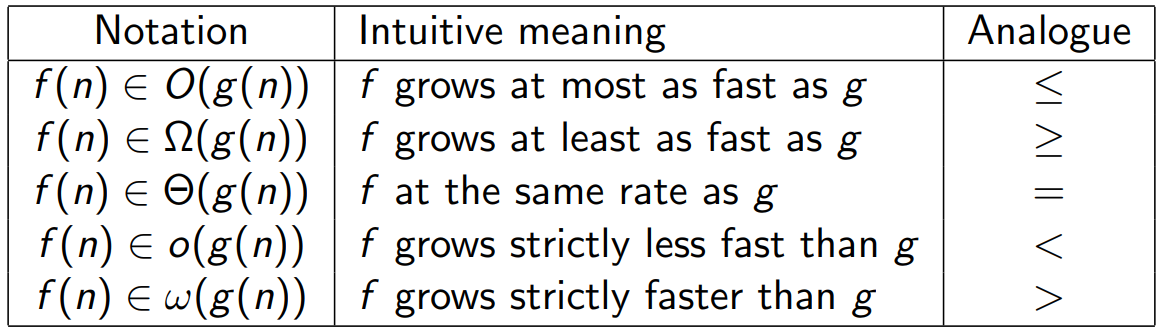
\includegraphics[width=8cm]{big-o-definition.png}
        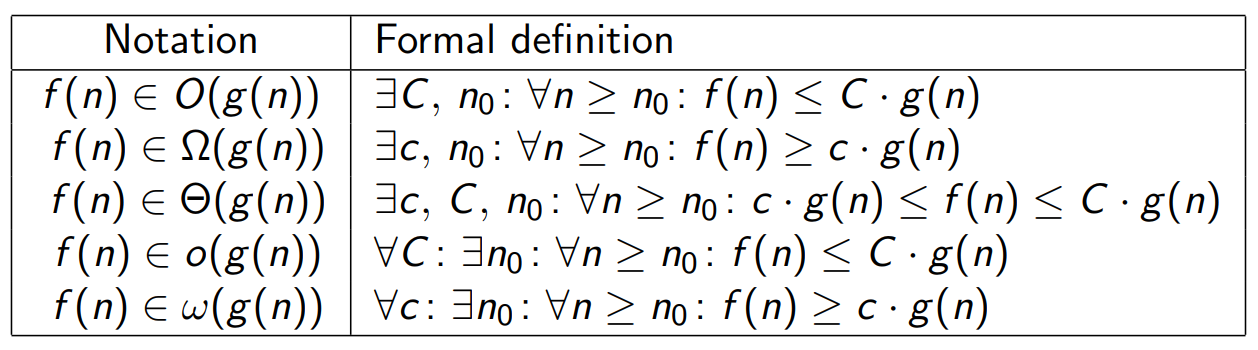
\includegraphics[width=8cm]{big-o-formal.png}
    \end{minipage}
};
%------------ Big O Header ---------------------
\node[fancytitle, right=10pt] at (box.north west) {Big O};
\end{tikzpicture}

%------------ Interval Scheduling ---------------
\begin{tikzpicture}
\node [mybox] (box){%
    \begin{minipage}{0.3\textwidth}
    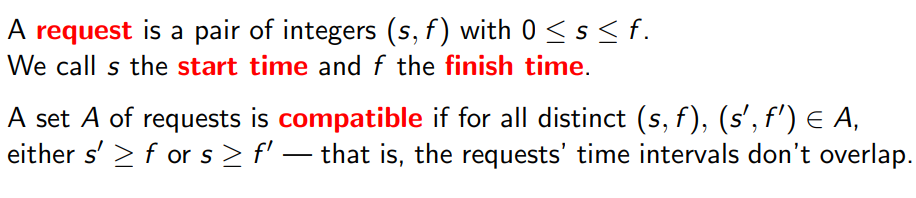
\includegraphics[width = 8cm]{req-comp-def.png}
    \hline
    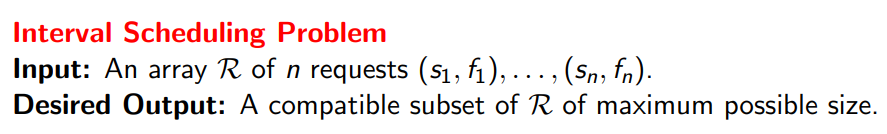
\includegraphics[width = 8cm]{interval-scheduling-problem.png}
    \hline
    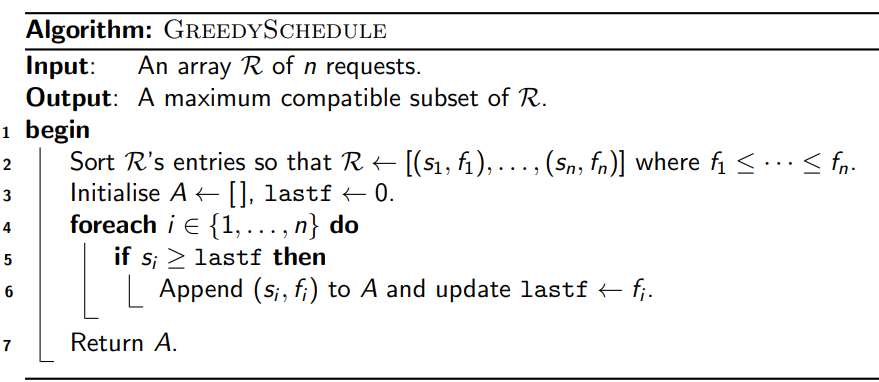
\includegraphics[width=8cm]{greedy-schedule-pseudo.png}
    \textbf{Complexity:} \\
    Step 2 takes O(n log n) \\
    Steps 3–6 all take O(1) time and are executed at most n times. \\
    $\therefore total running time = O(n log n) + O(n) · O(1) = O(n log n).$ \\
    \hline
    interval scheduling proofs 
    \end{minipage}
};
%------------ Interval Scheduling Header ---------------------
\node[fancytitle, right=10pt] at (box.north west) {Interval Scheduling};
\end{tikzpicture}







%------------ ODE Content ---------------
\begin{tikzpicture}
\node [mybox] (box){%
    \begin{minipage}{0.3\textwidth}
    \small{
    	\begin{tabular}{lp{4cm} l}
		\textit{1st Order Linear} & Use integrating factor,
        \\ & $I = e^{\int P(x) dx}$ \\ \hline
		\textit{Separable:} & $ \int P(y) dy/dx = \int Q(x) $ \\ \hline
		\textit{HomogEnEous:} & $ dy/dx = f(x,y) = f(xt,yt) $ \\ &
        sub $ y = xV $ solve, then sub $ V = y/x $ \\ \hline
        \textit{Exact:} & If $ M(x,y) + N(x,y)dy/dx = 0 $ and $ M_y = N_x $ i.e. $ \langle M,N \rangle = \nabla F $ then $ \int_x M + \int_y N = F $ \\ \hline
        \textit{Order Reduction} & Let $ v = dy/dx $ then check other types \\ 
        &\textit{If purely a function of y, }$\frac{dv}{dx} = v\frac{dv}{dy}$\\
        \hline
        \textit{Variation of Parameters:} & When $y''+a_1y'+a_2y = F(x)$ \\
        & $F$ contains $\ln x$, $\sec x$, $\tan x$, $\div$ \\ \hline
        \textit{Bernoulli} & $y' + P(x)y = Q(x)y^n$ \\
        & $\div y^n$ \\
        &$y^{-n}y'+P(x)y^{1-n}=Q(x)$ \textit{Let }$U(x) = y^{1-n}(x)$ \\
        &$\frac{dU}{dx}=(1-n)y^{-n}\frac{dy}{dx}$ \\
        &$\frac{1}{1-n}\frac{du}{dx} + P(x)U(x) = Q(x)$ \textit{solve as a 1st order} \\ \hline
        \textit{Cauchy-Euler} &$x^ny^n + a_1x^{n-1}y^{n-1} + \cdots + a_{n-1}y^{n-2}+a_ny = 0$ \\
        &guess $y = x^r$ \\
        \textit{3 Cases:} \\
        \textit{1) Distinct real roots} &$y = ax^{r_1}+bx^{r_2}$ \\
        \textit{2) Repeated real roots} &$y = Ax^r + y_2$ \\
        &\textit{Guess} $y_2 = x^ru(x)$ \\
        &\textit{Solve for $u(x)$ and choose one ($A=1, C=0$)} \\
		\textit{3) Distinct complex roots} &$y=B_1x^a \cos (b \ln x) + B_2x^a\sin (b \ln x)$
	\end{tabular}}
    \end{minipage}
};
%------------ ODE Header ---------------------
\node[fancytitle, right=10pt] at (box.north west) {ODEs};
\end{tikzpicture}

%------------ Laplace Transforms Content ---------------
\begin{tikzpicture}
\node [mybox] (box){%
    \begin{minipage}{0.3\textwidth}
    $L[f](s) = \int_0^{\infty} e^{-sx}f(x)dx $\\
    
    \small{
    	\begin{tabular}{lp{4cm} l}
        $f(t) = t^n, n \geq 0 $ &$F(s) = \frac{n!}{s^{n+1}}, s > 0 $ \\
        $f(t) = e^{at}, a \textit{ constant}$ & $ F(s) = \frac{1}{s-a}, s > a$ \\
        $f(t) = \sin{bt}, b \textit{ constant}$ & $ F(s) = \frac{b}{s^2 + b^2}, s > 0$ \\
        $f(t) = \cos{bt}, b \textit{ constant}$ & $ F(s) = \frac{s}{s^2 + b^2}, s > 0$ \\
        $f(t) = t^{-1/2}$ & $F(s) = \frac{\pi}{s^{1/2}}, s > 0$ \\
        $f(t) = \delta(t-a)$ & $F(s) = e^{-as}$ \\
        $f'$ & $L[f'] = sL[f] - f(0)$ \\
        $f''$ & $L[f''] = s^2 L[f] - sf(0) - f'(0)$ \\
        $L[e^{at}f(t)]$ & $L[f](s-a)$ \\
        $L[u_a(t)f(t-a)]$ & $L[f]e^{-as}$ 
        \end{tabular}}
    \end{minipage}
};
%------------ Laplace Transforms Header ---------------------
\node[fancytitle, right=10pt] at (box.north west) {Laplace Transforms};
\end{tikzpicture}

%------------ Vector Spaces ---------------
\begin{tikzpicture}
\node [mybox] (box){%
    \begin{minipage}{0.3\textwidth}
    $v_1, v_2 \in V$\\
    1. $v_1 + v_2 \in V$ \\
	2. $k \in \mathbb{F}, kv_1 \in V $ \\
	3. $ v_1 + v_2 = v_2 + v_1 $ \\
	4. $(v_1 + v_2) + v_3 = v_1 + (v_2 + v_3) $ \\
	5. $\forall v \in V, 0 \in V \mid 0 + v_1 = v_1 + 0 = v_1$ \\
    6. $\forall v \in V, \exists -v \in V \mid v + (-v) = (-v) + v = 0 $ \\
    7. $\forall v \in V, 1 \in \mathbb{F} \mid 1*v = v$ \\
    8. $\forall v \in V, k,l \in \mathbb{F}, (kl)v = k (lv)$ \\
    9. $\forall k \in \mathbb{F}, k(v_1 + v_2) = kv_1 + kv_2$ \\
    10. $\forall v \in V, k,l \in \mathbb{F}, (k+l)v = kv + lv$
    \end{minipage}
};
%------------ Vector Space Header ---------------------
\node[fancytitle, right=10pt] at (box.north west) {Vector Spaces};
\end{tikzpicture}
\end{multicols*}
\end{document}


Contact GitHub API Training Shop Blog About
© 2016 GitHub, Inc. Terms Privacy Security Status Help